\documentclass[a4paper]{article}
\usepackage{graphicx}

\title{Evry Programmeringsuppgift}
\author{Tim Mickelson}
\date{05/04/2014}

\begin{document}
\maketitle

\newpage

\section{Introduction}
The purpose of this documentation is to describe the approuch of resolving the programming assigment found in the \textit{pdf} document \textit{Programmeringsuppgift} provided by Evry~\cite{pdf}.

\section{The Problem}
The programming challenge consists of reading textual documents and giving \textit{points} for documents and it's containing words. The points are then presented to the standard output as requested in the
document \textit{Programmeringsuppgift}.

\section{Rules}
The rules as interpretted by me are:
\begin{enumerate}
	\item All words shorter then 3 characters and longer then 20 will not be considered, not even when counting the ammount of words in the document.
	\item All words of the lenght 3 characters are counted but not given points.
	\item All words between the length of 4 and 10 are \textit{short words} and always given at least one point.
	\item All words between 10 and 20 letters are \textit{long words} and are encounted for only if the contain the character \textit{"-"} otherwise they are totally ignored.
	\item If the document contains more then 100 words (short and long words with \textit{"-"}) then the short words get 2 points and the long 1 point.
	\item If the document contains more then 1000 words (short and long words with \textit{"-"}) then all words with double letter get one more point.
\end{enumerate}

\section{Usage}
The program is compiled with JDK 1.7.0 and Maven 3.0.1. Usage is quite simpe:

\begin{verbatim} 
$ java -jar evry-mickelson.jar [option] [file]
\end{verbatim} 

\begin{itemize}
	\item \textit{option} - Flag -f for file input or -d for directory input.
	\item \textit{file} - Absolute filename or directory.
\end{itemize}

\section{Technical Approach}

\begin{figure}
	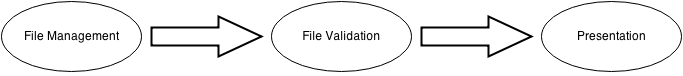
\includegraphics[scale=0.5]{evry-mickelson.png}
	\caption{Flow diagram}
	\label{fd}
\end{figure}

The problem is roughly divided in three phases as in Figure~\ref{fd}. Each phase has a corresponding class described below - \textit{see Figure~\ref{cd}}. The provided source code is well documented, but this documentation should give a rough description of the implementation.

\begin{figure}
	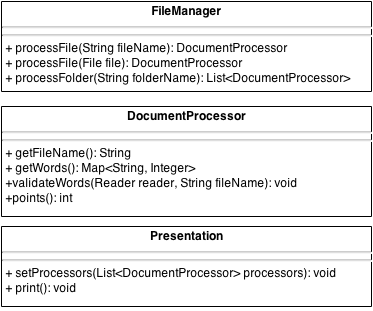
\includegraphics[scale=0.5]{cd.png}
	\caption{Class Diagram}
	\label{cd}
\end{figure}

The three classes 

\newpage

\begin{thebibliography}{99}
	\bibitem{pdf}Anders Dannqvist\emph{Programmeringsuppgift} EVRY Consulting AB, 2014
\end{thebibliography}

\end{document}
